§§ מחשבים עתיקים ולידתה של ליספ

שפת LISP (ראשי תיבות דו- וארבע שלביים של \E|LIst ProceSsing|), הייתה, יחד עם
שפת Fortran (ראשי תיבות תלת- ודו-שלביים של \LR{FORmula TRANslation}), אחת משתי
שפות התכנות העיליות הראשונות. פיתוחה של ליספ החל באוניברסיטת MIT לפני יותר
משישים שנה בהובלתו של ג'ון מקארת'י (\E|McCarthy|), מחלוצי הבינה המלאכותית.

שנים רבות לאחר מכן, יתקשה מקארת'י להיזכר מתי בדיוק הופעלה ליספ לראשונה.
בדיקה "ארכיאולוגית" של מסמכים ישנים מגלה כי כבר בשנת 1960 נעשה שימוב בגירסה
ראשונה של ליספ, \E|LISP~I| שמה, כבר שימשה ליישומי חשבון דיפרנציאלי ואינטגרלי,
תיאוריה של מעגלים חשמליים, לוגיקה מתימטית ובינה מלאכותית. עוד עולה כי המאמץ
למימוש השפה החל בשנת 1958. כבר באותה שנה הציג מקארת'י לראשונה מזכר המתאר את
ליספ, לא כשפת תכנות, אלא כתחשיב מתמטי לתיאור "הגיוני" (\E|"sensible”|) של
אלגוריתמים. תחשיב זה של מקארת'י התבסס על תחשיב מתימטי אחר: תחשיב ה-$λ$
\E|(lambda calculus)| שפיתח אלונזו צ'רץ' (\E|Church|) בשנת 1936.

בימים ההם נדרש מאמץ משמעותי כדי לממש את התחשיב המתימטי של מקארת'י כשפת תכנות
הפועלת על מחשב: תכניות נכתבו אז בשפת מכונה, הוזנו למחשב על כרטיסים מנוקבים,
והפלט שלהן התקבל על מדפסות איטיות. המחשב המתקדם ביותר באותה עת היה \E|IBM~704|,
מחשב הבנוי משפופרות ריק (מאלו שאפשר לראות במכשירי טלוויזיה ורדיו עתיקים), מחשב
שתפס אמנם אולם שלם, אך גודל הזיכרון שעמד לרשותו היה פחות מ-20 קילובית, והוא היה
איטי בכמעט פי עשרת אלפים מטלפון סלולרי מיושן כדוגמת \E|Samsung~S2|.

לעומת זאת, לא היה קשה לממש את ליספ באמצעות עצמה. מקארת'י הציג לראווה את כוחה
של ליספ בכך שכתב בה פונקציה (רקורסיבית אמנם, אך רחוקה מלהיות מסובכת),
\begin{equation} \label{eq:eval}
  \text{eval}(ℓ, a),
\end{equation}
אשר קיבלה כפרמטר תכנית ליספ כלשהי~$ℓ$, וביצעה את~$ℓ$ תוך שימוש ב-$a$, הפרמטר
האחר ל-\E|eval|, כ-"סביבה" שבה יש לבצע את~$ℓ$. הסביבה היא רשימת ההגדרות בהן~$ℓ$
יכולה להשתמש. לשם ביצוע תכנית נתונה~$ℓ$, יש להפעיל את-\E|eval| על~$ℓ$
ועל~$a$ המציין רשימת הגדרות ריקה. הפעלות רקורסיביות של \E|eval| תהיינה על חלקים
שונים של~$ℓ$, ועל רשימת ההגדרות אשר נוצרו במהלך החישוב, שהרי יצירה זו מתרחשת כל
אימת שמועברים ארגומנטים בקריאה לפרוצדורה או לפונקציה: שם הפרמטר מוגדר להיות
ערכו של הארגומנט.

מקארת'י הראה שכאשר \E|eval| מופעלת על תכנית~$ℓ$ ועל סביבה ריקה היא
תבצע את~$ℓ$ ממש כפי שמימוש של ליספ על מחשב היה מבצע אותה. דא עקא, שמימוש כזה
טרם היה בנמצא, ובנייתו הייתה רק בראשיתה: החוקרים שעמלו על כך עדיין תהו
כיצד ניתן לממש את ליספ כך שתוכל לרוץ באופן סביר על תשתית המחשוב הרעועה שעמדה
לרשותם. כך למשל, מדי כשמונה שעות בממוצע היה המחשב מושבת לתיקון עקב כשל באחת
מבין שפופרות הריק מהן הוא בנוי. על כך נוספה בעית קצב העיבוד שהיה איטי כל כך
שהמהדר (אשר כבר מומש) של פורטרן לא תמיד הצליח לסיים את פעולתו טרם שיוזעק טכנאי
לתיקון תקלה שהתגלתה במחשב.

מסיבה זו, הצעדים הראשונים במימוש של ליספ היו בגדר גישושים: החוקרים נהגו לבחור
תכניות ליספ קצרות, לתרגם אותן ידנית לתכניות בשפת מכונה, ולבחון את דרך פעולתם של
התרגומים שנוצרו. פריצת הדרך חלה כאשר אחד החוקרים, סטיב ראסל (\E|Russel|),
הבחין שניתן להשתמש בפונקציה \text{eval} שכתב מקארת'י כדי לממש את ליספ על מחשב
של ממש. במקום לבנות מימוש כללי של ליספ, כזה המסוגלת להתמודד עם \ע|כל| תכנית
ליספ כלשהי, מספיק לממש תכנית ליספ \ע|אחת|, הלא היא הפונקציה \E|eval|!

בליספ, כל תכנית היא פונקציה, וכל פונקציה היא תכנית. הפונקציה \E|eval| היא לכן
תכנית המסוגל לטפל בכל תכנית ליספ שהיא. ראסל תרגם את הפונקציה \E|eval| מליספ
לשפת מכונה, ואחר כך השתמש בתרגום זה והוסיף עליו מעט כדי לממש את ליספ. המימוש
היה כ\ע|אינטרפרטר|: תכנית הקוראת שורה מהקלט, מפרשת אותה כתכנית ליספ, מבצעת
אותה ומדפיסה את תוצאת החישוב.

\begin{figure}[H]
\centering
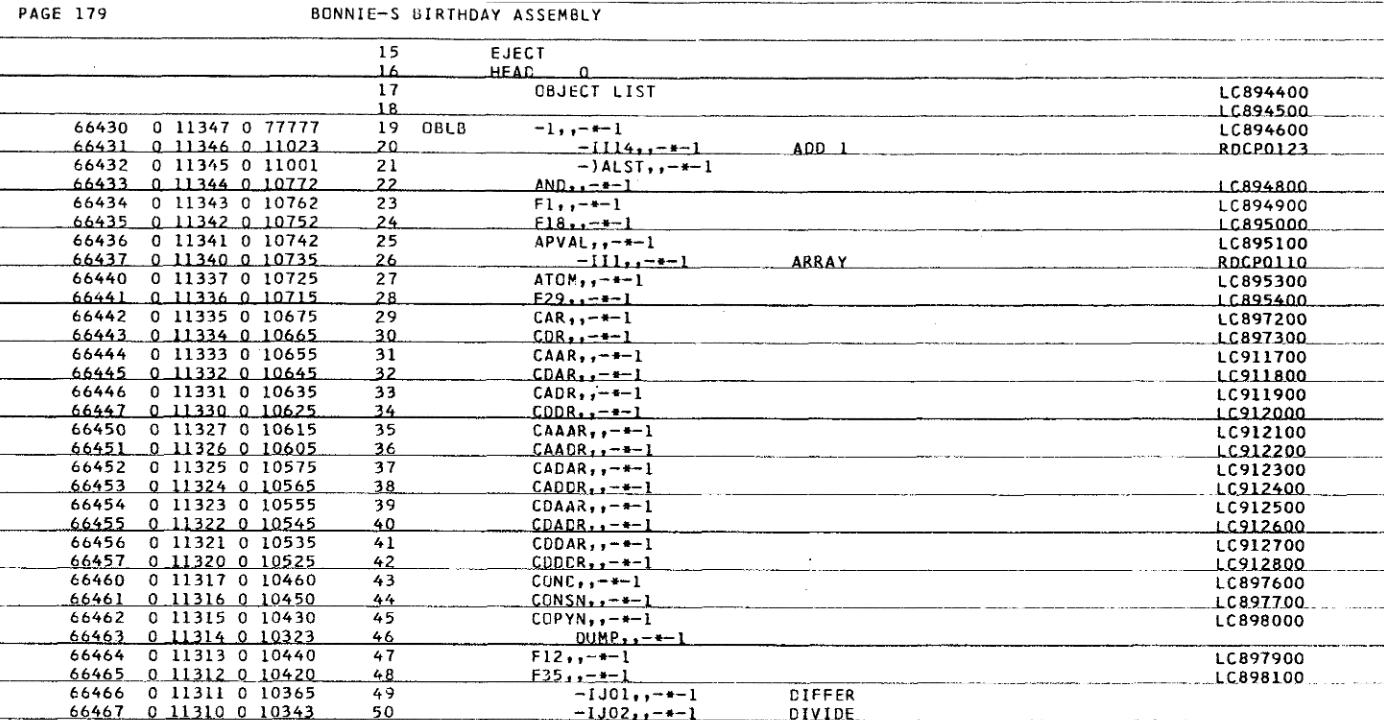
\includegraphics[width=0.45\textwidth]{lisp-assembler2}
\qquad
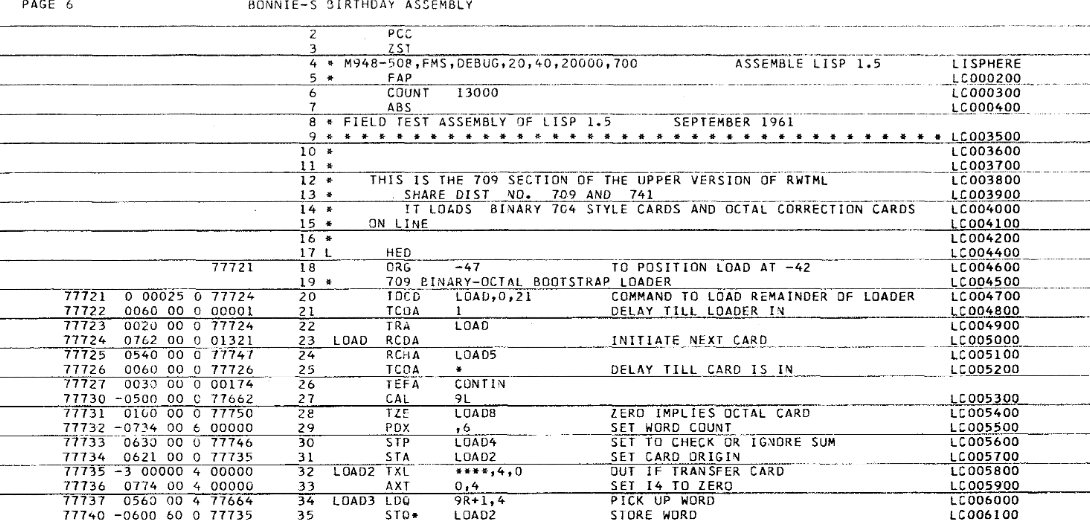
\includegraphics[width=0.45\textwidth]{lisp-assembler1}
\כיתוב|קטע מהתכנית בשפת מכונה שמימשה לראשונה את ליספ|
\תגית|איור:מימוש|
\end{figure}

\פנה|איור:מימוש| מציג קטע מהתכנית בשפת מכונה שנכתבה על ידי ראסל וחבריו כדי לממש
את eval ובאמצעותה את ליספ.

§§ \RL{נסיקתה (וצניחתה) של ליספ}

לאחר מימושה, זכתה ליספ לענין גובר והולך: מתכנתים רבים העדיפו את האלגנטיות
והתמציתיות של ליספ, על פני המסורבלות של שפת פורטרן ושפות תכנות אחרות, ולו גם
במחירה של יעילות, שכן מעצם טיבה כשפה שאינה יכולה לעבור הידור מלא, הרצה של
תכניות בליספ איטית יותר מאשר תכניות שתורגמו משפה עילית לשפת מכונה.

\lstdefinestyle{interaction}{%
  style=display,
  frame=none,
  language=Pascal,
  backgroundcolor=\color{purple!10},
  deletekeywords={to,do,of,and,then,for},
}

בשנות השישים והשבעים שימשה השפה לפיתוחן של כמה תכניות פורצות דרך, אשר עירבו בהן
מידה זו אחרת של בינה מלאכותית: למשל,מאקסימה (\E|Macsyma| ואחר כך \E|Maxima|)
הייתה התכנית הראשונה לחישוב מתמטי סימבולי (ולא נומרי) כגון חישובי נגזרות
ואינטגרלים או פתרון של משוואות דיפרנציאליות. למשל, חישוב במקסימה של האינטגרל
הלא מסוים
\begin{equation}
  \label{eq:indefinite}
  ∫\sin³(x)\, dx=\frac{\cos³(x)}3- \cos(x)
\end{equation}
ואת האינטגרל המסוים
\begin{equation}
  \label{eq:definite}
  ∫₀^π e^x\cos²(x),dx=\frac{3 (e^π-1)}{5}
\end{equation} נעשה זאת כמתואר ב\פנה|איור:מאקסימה|.

\begin{figure}[H]
\centering
\begin{LTR}
  \lstinputlisting[style=interaction]{Forests/MAXIMA.txt}
\end{LTR}
\caption[שימוש במאקסימה לחישוב אינטגרלים]{שימוש במאקסימה לצורך חישוב האינטגרל הלא
מסוים~$∫\sin³(x)\,dx=\frac{\cos³(x)}3-\cos(x)$ והאינטגרל
המסוים~$∫₀^π e^x\cos²(x),dx=\frac{3(e^π-1)}{5}$}
\תגית|איור:מאקסימה|
\end{figure}
השיח בין המשתמש ומאקסימה באיור נפתח בסידרת ה\ע|תווים| (\E|characters|)
\begin{LTR}
\begin{lstlisting}[style=interaction,backgroundcolor=\color{white}]
(%i1)
\end{lstlisting}
\end{LTR}

סידרה זו היא היא ה\ע|זרז| (\E|prompt|) שמציגה תכנת מאקסימה למשתמש בה: בהצגת
הזרז, מתבקש המשתמש להזין ביטוי מתימטי עליו מאקסימה נדרשת לפעול. ביטוי זה יסומן
כקלט מספר~1, ומכאן הכתיב (\mini{i1}).

הביטוי שמזין המשתמש בתגובה לזרז הוא \E|\mini{integrate(sin(x)³,x)}| הוא
האינטגרל אותו על מאקסימה לחשב. בתגובה, מחשבת מאקסימה את האינטגרל, ומדפיסה אותו,
תוך שהיא מסמנת אותו ב-
\begin{LTR}
\begin{lstlisting}[style=interaction,backgroundcolor=\color{white}]
(%o1)
\end{lstlisting}
\end{LTR}
 כלומר פלט מספר~1. חישוב האינטגרל~$∫₀^πe^x\cos²x\,dx$ נעשה אחר כך, כאשר הקלט
 והפלט מסומנים כמספר~2.

ישום בינה מלאכותית מובהק בליספ הוא "אלייזה" (\E|ELIZA|), תכנית המחשב הראשונה
שהייתה מסוגלת לנהל שיח עם משתמש בדומה לצ'אטבוט מודרני. אלייזה ניסתה לדמות בשיחה
את תפקיד הפסיכיאטר או הפסיכותראפיסט ודו-שיח עמה נראה, לדוגמה, כמופיע
ב\פנה|איור:אלייזה|.

\begin{figure}[H]
\centering
\begin{LTR} \scriptsize
  \lstinputlisting[style=interaction]{Forests/ELIZA.txt}
\end{LTR}
\כיתוב|קטע משיחה בין תכנת אלייזה ובין משתמש|
\תגית|איור:אלייזה|
\end{figure}

ELIZA הייתה כה מוצלחת כצ'אט בוט, שכמה מהמשוחחים עמה נפתו לחשוב שהם משוחחים עם
פסיכיאטרית היושבת במקום אחר ומשוחחת עימם באמצעות המחשב.

שפת ליספ שימשה גם לפיתוח \E|DART|, תכנת לוגיסטיקה של משרד הבטחון האמריקאי, אשר
ניהלה את שינוע של הכוחות, הציוד והתחמושת במבצע סופת המדבר (\E|desert storm|),
ולמעשה איפשרה אותו. היא שימשה לכתיבת תכנה הסוחרת עצמונית בבורסה, לכתיבת
\E|Grammarly|, תוסף מפורסם לדפדפנים המציע תיקוני הגהה ודקדוק במהלך הכתיבה, ועוד
ועוד שימושים רבים, מגוונים, ומתוחכמים.

חשיבותה של ליספ עלתה עד כדי כך שבמשך כל שנות השבעים, השמונים, ותחילת התשעים של
המאה הקודמת, נבנו מחשבים יעודיים, \E|Lisp machines| אשר הארכיטקטורה שלהם תוכננה
בעבור במיוחד לשם ביצוע יעיל של תכניות ליספ. ייצור המכונות הללו חדל כאשר התברר
כי הן אינן מצליחות להתחרוות בעליה המעריכית בביצועיהם של מחשבים לשימוש כללי.

במהלך השנים, נולדו (ומתו) ניבים רבים לליספ שהרחיבו ושינו בהרבה את ההגדרה
המקורית של מקראתי. בשנת 1984 אוחדו רבים מהניבים הללו לכדי הגדרה של שפה אחת
הידועה בשם \E|Common Lisp|. ניבים נפוצים אחרים כוללים את Emacs Lisp (המשמשת
כשפת סקריפטים בעבור עורך הקבצים (\E|text editor|) הידוע בשם \E|Emacs|),
AutoLisp (המשמשת כשפת סקריפטים בתכנת \E|AutoCad|), \E|Scheme|, \E|Clojure|,
ואפילו שפת התכנות \E|Dylan|, אשר למרות הדקדוק שהדקדוק שלה שונה בתכלית מזה של
ליספ, היא עדיין מבוססת עליה.

החדשנות שביסודה של ליספ שוחזרה שוב ושוב בשפות תכנות מודרניות לרוב, ובהן
פיית'ון, \E|Ruby|, סקאלה, \E|Perl|, \E|Swift|, \E|Standard ML|, \E|Lua|,
\E|NIM|, ועוד שפות אחרות. נראה כי הלבוש החדש של אותם רעיונות לא הועיל למי
שהציגה אותם לראשונה. נראה כי השימוש בליספ דועך, ומספר הפרויקטים המסחריים החדשים
בליספ הוא ככל הנראה אינו גדול.

§§ מליספ אל מיני-ליספ

הענין שלנו בליספ אינו רק מפני חשיבות מסחרית, תרבותית, מעשית, היסטורית, או
עכשווית כלשהי, או מפני מידת השימוש בה. יש יתרון אינטלקטואלי בלימוד ליספ: השפה
מדגימה בתמציתיות עקרונות ומושגים מרכזיים המופיעים שוב ושוב כמעט בכל שפת תכנות:
עיבוד רשימות ורקרוסיה, חישוב סימבולי וביטויי~\E|S|, אינטרפטציה והידור,
אוניברסליות ואלגנטיות, האבחנה בין שם למשוים, הקישור בין שם למשויים באורח דינמי
או סטטי (הקרוי גם קישור לקסיקלי), סביבה (\E|environment|) הכוללת אוסף של
הגדרות, ומנגד, טווח (\E|scope|) של הגדרות, פונקציות טהורות וכאלו שאינן טהורות,
שיערוך, עצי שיערוך (הקרויים גם עצי דקדוק אבסטרקטי), אסטרטגיית שיערוך, סדר
שיערוך, ותכונת צ'רץ' רוסר, ועוד.

אנו נפגוש עקרונות ומושגים אלו כאשר נשחזר את הדרך שבה מומשה ליספ לראשונה: לשם
כך, נגדיר את שפת התכנות התיאורטית \ע|מיני-ליספ|, שהיא ניב רזה של ליספ.
ב\פנה|פרק:מימוש| נממש במיני-ליספ את הפונקציה \text{eval} עבור מיני-ליספ. המימוש
הזה הינו פשוט דיו כדי שיהיה ברור שניתן לממש אותו בקלות על שפת תכנות מודרנית.
המימוש הראשון של מיני-ליספ נבנה (בידי מחבר מסמך זה) ממש כשם שנבנה המימוש הראשון
של ליספ:
תרגום ידני של \text{eval}, כפי שנכתבה במיני-ליספ, לשפה אחרת, אלא
שבמיני-ליספ התרגום היה לשפה תכנות עילית שנבחרה כמתאימה ביותר לכך†{%
מדובר בשפה המוסיפה על שפת~\E|C++| תוספות קלות אך גם גזירות קשות בדבר
המנעות משימוש במרבית התכונות של שפה זו.
}
ולא לשפת מכונה כפי שנאלץ ראסל לעשות. בכל זאת, בניסיון להתחקות אחרי הקושי
במימוש הראשוני של ליספ, המימוש של מיני-ליספ מגביל עצמו גם הוא לזיכרון בגודל של
כמה עשרות קילובית זיכרון.

§§ ביטויי~\E|S|
\תגית|פרק:S0|

התחשיב של מקארת'י, ובעקבותיו שפת ליספ וגם שפת מיני-ליספ, משתמשים במבנה מתימטי
יסודי אחד: \textbf{ביטוי~\E|S|} (\E|S-Expression|), או \textbf{ביטוי סימבולי}
(\E|symbolic expression|). כל התכניות והערכים בשפת ליספ הן ביטויי~\E|S|.

המילה "סימבולי" מדגישה את העובדה כי אין מדובר בביטוי מתמטי
כגון~$13+41/2$ או אלו המופיעים ב-\ref{eq:indefinite} ו-\ref{eq:definite}, בהם
משמעות הסימנים ידועה וברורה. אלא בביטוי \E|כללי| המכיל סמלים שאין להם
משמעות כשל עצמם.

הגדרה מתימטית מדויקת של ביטויי~\E|S| מופיעה ב\פנה|פרק:S|. עד אז, נדמה
ביטויי~\E|S| כמבנה נתונים פשוט: עץ בינארי מלא (כלומר עץ שדרגת כל צומת בו היא~0
או~2), ואשר העלים בו (כלומר הצמתים שדרגתם~0) נושאים תגיות. אין תגיות בצמתים
הפנימיים (הצמתים שדרגתם~2).

לדוגמה, בעץ שב\פנה|איור:מלא| יש שני צמתים פנימיים, אשר אינם נושאים תגית, ושלושה
עלים מתויגים, שניים מהם בתגית~$a$, והשלישי בתגית~$b$.

\begin{figure}[H]
  \centering
  \begin{LTR}
 \begin{quote}
   \scriptsize
  \center
  \Forest{s tree [{},cons [$a$,atom],[{},cons [$b$,atom] [$a$,atom]]] }
\end{quote}
\end{LTR}
  \כיתוב|עץ בינארי מלא בו עלים נושאים תגיות|
  \תגית|איור:מלא|
\end{figure}

ישנם שני סוגים של ביטויי~\E|S|: ביטוי~\E|S|\ הוא ע|אטומי| אם הוא עץ מנוון אשר
בו צומת אחת בלבד: עלה הנושא תגית כלשהי. כל ביטוי~\E|S| אחר נקרא ביטוי
\ע|מורכב|, והעץ המתאר אותו מכיל צומת פנימי אחת לפחות. העץ שב\פנה|איור:מלא| הוא
ביטוי~\E|S| מורכב.

ביטוי סימבולי אטומי, כשמו כן הוא: בלתי ניתן לחלוקה. ביטוי סימבולי אטומי אינו
מכיל תתי ביטוים. לעומת זאת, כל ביטוי סימבולי מורכב נבנה משני תתי-ביטוים,
המתאימים לתתי העצים הימני והשמאלי של העץ המתאר את הביטוי. \פנה|איור:שבור| מראה
את שני תתי העצים של העץ שראינו ב\פנה|איור:שבור|. הביטוי הסימבולי המתאים לעץ
מתפרק כך לשני ביטוים סימבוליים: האחד אטומי והאחר מורכב.

\begin{figure}[H]
\caption[פירוק עץ בינארי לשני תתי עצים]{פירוק העץ הבינארי המלא שב\פנה|איור:מלא|
      לשני תתי העצים שלו, שאף הם בינאריים ומלאים}
\תגית|איור:שבור|
  \scriptsize
  \center
  \input Forests/decomposing-S-into-two.tikz
\end{figure}

§§ שיערוך וביטויי S

כאמור, כל תכנית~$ℓ$ בליספ מיוצגת כביטוי~\E|S| \[
  s=s(ℓ).
\] הרצה, ביצוע או הפעלה של~$ℓ$ פירושם שיערוך של של הביטוי~$s$. שני צעדים
מושגיים בשיערוך:
\אבגד
✦ \ע|פרשנות|, כלומר מציאות המשמעות של הסימבולים שבביטוי. אלו הן התגיות המופיעות
בעליו של הביטוי. יתכן כי למספר תגיות ישנה משמעות קבועה. אולם, בדרך כלל נעזר
תהליך השיערוך בטבלת עזר המעניקה משמעות לתגיות. לטבלה זו קוראים \ע|טבלת סמלים|
(\E|symbol table|), מונח המופיע שוב ושוב כמעט בכל שפות התכנות. משמעות התגיות
המקבלת מטבלת הסמלים יכולה להיות ערכים שהם ביטויי-\E|S| "פשוטים", או
ביטויי-\E|S| שהם פונקציות אשר אותן יש להפעיל במסגרת החישוב.

✦ \ע|חישוב| ערכו של הביטוי בהתאם לפרשנות זו החישוב נעשה בדרך כלל באמצעות הפעלה
של פונקציות על פרמטרים. כמו צעד הפרשנות גם צעד החישוב יכול להיכשל, ואזי גם
השיערוך נכשל. אחרת, תוצאת השיערוך היא תוצאת החישוב שנעשה בצעד זה.
===

(שיערוך מתקיים באופן זה או אחר ברוב שפות התכנות. בליספ, הפרשנות והחישוב
משולבים זה בזה. אולם אין הדבר תמיד כך: למשל, בשפת התכנות פסקל הפרשנות נעשית
בזמן ההידור, והחישוב נעשה בעת ההרצה לאחר ההידור. בשפת Java לעומת זאת, מרבית
הפרשנות נעשית בזמן ההידור, מקצתה אך חלקה נעשה בבל פעם בה נטען לביצוע חלק מחלקי
התכנית, וחלקה האחר בזמן ההרצה ממש.)

השיערוך בליספ מופעל על ביטוי~\E|S|. אם השיערוך אינו נכשל, אזי תוצאת השיערוך גם
היא ביטוי~\E|S|, שהוא, במרבית המקרים, שונה מהביטוי הנתון. במילים אחרות, שיערוך
הוא טרנספורמציה (העשויה להיכשל) המעתיקה ביטויי~\E|S| אל ביטויי~\E|S|. פעולת
השיערוך אינה מבצעת רק את הטרנספורמציה הזו, שכן במסגרת השיערוך יתכנו עדכונים
לטבלת הסמלים הנותנת משמעות לתגיות.

לא רק תכניות הן ביטויי~\E|S|. כל הנתונים בשפת ליספ גם הם ביטויי~\E|S|. תכנית
בשפת ליספ היא פונקציה המקבלת אפס או יותר פרמטרים, שהם כולם ביטויי~\E|S|, פועלת
על ביטוי~\E|S| אלו ומחזירה ביטוי~\E|S| המחושב מפרמטרים אלו. כיוון שסדרת
הפרמטרים לפונקציה מועברת לה כפועל כביטוי~\E|s| יחיד המייצג את הסידרה, הרי כל
פונקציה בליספ מייצגת טרנספורמציה של ביטויי~\E|S|.

במתימטיקה המונח "פונקציה" הוא מה שקרוי גם \ע|פונקציה שלמה|, כלומר מיפוי של
\ע|כל| ערך של קבוצת התחום לערך כלשהו של קבוצת הטווח. לעומת זאת \ע|פונקציה
חלקית| היא כזו אשר בה המיפוי הינו חלקי בלבד, ויתכנו ערכים בקבוצת התחום אשר
עבורם המיפוי אינה מוגדרת. אנו נשתמש במונח פונקציה כדי לתאר פונקציות כפי שהן
מצויות בליספ, בפסקל, ב-\E|C|, כמו גם בשפות תכנות אחרות. לדידנו, פונקציה היא
מקטע של תכנית המתאר כיצד להמיר ערך (או ערכים) לערך אחר. המיפוי אותו מייצגת
פונקציה אינו, בדרך כלל, פונקציה במובן המתימטי של המונח.

ישנן פונקציות בליספ, כמו למשל פונקצית הזהות, שהן פונקציות שלמות. אולם, על דרך
הכלל, פונקציות בליספ הינן פונקציות חלקיות מקבוצת ביטויי ה-\E|S| אל עצמה.
החלקיות נובעת מהעובדה שתהליך המרת הערכים הנעשית בפונקציה עשויה להיכשל, עקב אחת
מבין שלוש סיבות: כישלון במציאת משמעות לתגית, כישלון בחישוב כתוצאה מביצוע פעולה
לא חוקית, וגם, התפתחות תהליך השיערוך לכדי חישוב שאינו מסתיים לעולם.

\פנה|פרק:שיערוך| בהמשך מתאר את אלגוריתם השיערוך, הידור לעומת אינטרפטציה בכלל,
ואת השיערוך בליספ, כפי שימומש במיני-ליספ ב\פנה|פרק:מימוש|.

§§ הפרדיגמה הפונקציונלית והומואייקוניות

לא זו בלבד שכל פונקציה של ליספ היא ביטוי~\E|S|, אלא גם שכל ביטוי~\E|S| הינו
בעצמו פונקציה בליספ, המייצגת טרנספורמציה (אשר עשויה להיכשל) של ביטויי~\E|S|.
(אמנם ביטויי~\E|S| שלא נבנו במבנה המיוחד של ביטוים המייצגים פונקציות, הם בדרך
כלל פונקציות מנוונות, הנכשלות עבור כל פרמטר שהוא.)

כיוון שכל פונקציה בליספ היא בעצמה ביטוי~\E|S|, אין בליספ הבדל של ממש בין
פונקציה המקבלת כפרמטרים ערכים "רגילים" ומחזירה ערך "רגיל" המחושב מערכים אלו,
ובין פונקציה המקבלת כפרמטרים פונקציות אחרות ומחזירה בתמורה פונקציה הבנויה
מפונקציות הללו. פרמטרים לפונקציה של ליספ יכולים להיות פונקציות, פונקציות
המקבלות כפרמטרים פונקציות, פונקציות המקבלות כפרמטרים פונקציות המקבלות כפרמטרים
פונקציות, וכו'.

היכולת של ליספ להעביר פונקציות כפרמטרים ולהחזיר אותן כתוצאה מחישוב, היא זו
המייחדת את הפרדיגמה הפונקציונלית. בפרדיגמה זו, אנו מוצאים פעמים רבות פונקציה
בשם \E|map| המפעילה פונקציה נתונה על איברי רשימה נתונה, כמו גם פונקציה בשם
\E|compose| המחזירה את ההרכבה של שתי פונקציות הניתנות לה כפרמטרים. בפרדיגמה זו
אין משתנים, פקודות הצבה (או אף לא כל פקודה אחרת). גם פרוצדורות או
לולאות לא נמצא בפרדיגמה הפונקציונלית. במקום כל אלו, הפרדיגמה הפונקציונלית
משתמשת בביטוים, פונקציות, ורקורסיה.

הפרדיגמה הפונקציונלית מתבססת על מספר פעולות יסודיות אותן ניתן לבצע על ערכים
המייצגים פונקציות: העברת פונקצית כפרמטר לפונקציה אחרת, קבלת ערך של פונקציה
מהפעלה של פונקציה אחרת, הרכבת פונקציות, ועוד. כל הפעולות הללו מתייחסות אל גוף
הפונקציה עצמה כקופסה שחורה. הפרדיגמה הפונקציונלית אינה כוללת בתוכה את הכוח
לפתוח קופסה זו: ולא ניתן בשפות פונקציונליות רגילות לבחון את התוכן של ערך מסוג
פונקציה, כלומר לבדוק כיצד פונקציה ממומשת או לשנות מימוש זה.

ליספ \ע|מוסיפה| על הפרדיגמה הפונקציונלית את היכולת לבצע טרנספורמציה של
פונקציות. קל לכתוב בליספ פונקציה המקבלת שלושה ביטויי~S המייצגים
פונקציות~$f$,~$g$ ו-$g'$, ואשר מייצרת מהם ביטוי~\E|S| המייצג פונקציה~$f'$ הדומה
לפונקציה הנתונה~$f$, אלא שכל קריאה של~$f$ ל-$g$ מוחלפת בפונקציה~$f'$ בקריאה
לפונקציה~$g'$. ניתן לממש בליספ טרנספורמציות אחרות של פונקציות לצורך שיפור
יעילות, איסוף מידע סטטיסטי לצורכי אופטימיזציה, ואפילו הידור של תכניות בליספ
לשפות תכנות אחרות.

אנו אומרים ששפת ליספ ניחנה בתכונה הידועה בשם \ע|הומואייקוניות|
(\E|homoiconicity|) לפיה ניתן מתוך השפה לבצע מניפולציה על תכניות הכתובות בשפה
כאילו היו הן נתונים. שפות אחרות שהן הומואייקוניות כוללות את פרולוג, \LR{Wolfram
Mathematica}, \E|Snobol| ו-\E|Julia|. לעומת זאת, שפות כמו~\CPL, פסקל,
ו-\E|Java|, כמו מרבית שפות התכנות אינן הומואייקוניות.

גם הפונקציה \E|eval| מנצלת את ההומואייקוניות: היא מקבלת כפרמטר ביטוי~S ומשערכת
אותו. אגב, כיוון ש-\E|eval| היא ביטוי~S בעצמה, הרי ניתן להפעיל אותה על עצמה.

העובדה שניתן לממש את ליספ באמצעות ליספ עצמה היא מעניינת, אך אין היא מפתיעה: כפי
שנראה בסופו של פרק זה, תכונה זו מתקיימת כמעט בכל שפת תכנות. בכל זאת, מי שאינו
מכיר את ליספ, ודאי יופתע אולי מהעובדה שהמימוש הזה הוא קצר ופשוט כל כך. כפי
שנסביר עוד בסוף הפרק, עובדה זו היא אכן עדות לאלגנטיות של שפת ליספ.


